\documentclass[12pt]{article}
% This first part of the file is called the PREAMBLE. It includes
% customizations and command definitions. The preamble is everything
% between \documentclass and \begin{document}.

\usepackage[margin=1in]{geometry}  % set the margins to 1in on all sides
\usepackage{graphicx}              % to include figures
\usepackage{amsmath}               % great math stuff
\usepackage{amsfonts}              % for blackboard bold, etc
\usepackage{amsthm}                % better theorem environments

\usepackage{rotating} % for sideway table
\usepackage{xcolor}
\usepackage{hyperref}
\hypersetup{
    colorlinks,
    linkcolor={red!50!black},
    citecolor={blue!50!black},
    urlcolor={blue!80!black}
}
\usepackage{cleveref} % Reference
\usepackage{enumitem} % nosep

\usepackage{array,tabularx}

% bibliography
\usepackage{natbib}
\bibpunct{(}{)}{;}{a}{}{,} % no comma between author and year

\title{Prospectus: The effect of corruption on FDI technological spillover}
\author{Anh Le}


\begin{document}
\maketitle

\section{Generalized Theory}
\subsection{Actor and choices}

The model has one strategic actor: a government official. This official has control over a certain endowment (e.g. market access, cheap labor) that is attractive to foreign firms.\footnote{I define \textit{foreign firms} as firms with over 50\% ownership belonging to private foreign individuals, companies, or organizations. In these firms, we are certain that the foreign owner has the majority stake and is responsible for the firm's action. This definition is common across business surveys and national laws, allowing us to collect a wide range of data.} Foreign firms that invest in the official's territory turn this endowment into profit via their productive activities. Firms then share the value added with the official in exchange for access to the endowment. 

Firms share the benefit with the official in the form of a two-good bundle: 1) technological spillover and, 2) private benefits (to the official). \textit{Technological spillover} is the beneficial effects of foreign firms' technological knowledge on the productivity and innovative ability of domestic firms. The official cares about the technological spillover of FDI because it is a crucial ingredient in improving total factor productivity and generating long-term growth, which in turn, brings electoral or career benefits. \textit{Private benefits} that firms offer to the official can come in many forms, both illegal (e.g. bribe, kickback) and legal (e.g. campaign finance contribution, informal network with foreign firms that leads to contracts for friends and families). The essence of the dissertation project is to determine how the official chooses the mix of these two goods, i.e. technological spillover and private benefit.

In this model, the firm does care about whether the official demands spillover or private benefits but only because firms have heterogeneous abilities in offering spillover and private benefits. For example, if a firm belongs to an industry where production is divisible, it is easier and less expensive for the firm to sub-contract local firms and create spillover. Similarly, if a firm comes from a country with little corruption, it may be less adept in dealing with the official, has to hire local agents, and thus find it more expensive to offer the same amount of private benefits than other firms that are familiar with corrupt dealings. I model this preference of firm via two parameters: the ``price'' of spillover and the ``price'' of private benefit, which the official has to consider when he demands one of the two goods from the firm. By doing so, my model is able to incorporate the firm's preference without introducing it as a strategic actor.

This model has two assumptions. First, I assume that offering spillover or private benefits does not affect the firm's utility other than through the bottom line. If we believe that firms are unlikely to have moral (or other non-financial) incentives to bring spillover or to withhold bribe, then this assumption is reasonable. 

Second, I assume that the firm is satisfied as long as its retained profit remains above the reservation level. The firm will not invest if and only if the official's demand reduces its profit to below this level. This assumption is reasonable according to the behavioral model of firms, in which firms are profit-satisficing instead of profit-maximizing \citep{Simon1959}. Granted, it is less defensible to build a model with one actor satisficing (the firm) while the other maximizing (the official). Therefore, in an extension to my project, I will model both actors as utility maximizing and use two-sided logit (TSL) to estimate their preferences. \citet{Logan1996a} has shown that the TSL corresponds to the game-theoretic college admissions model, a many-to-one matching problem that is relevant to how countries and FDI firms find their match.


\subsection{The trade-off between spillover and private benefits}

To induce spillover, governments frequently impose on foreign firms conditions such as forming a joint venture or local content requirement. These conditions constrain firms' options and their ability to optimally use their physical and management capital, reducing their revenue and profitability. Similarly, when firms are forced to offer private benefit to officials (e.g. bribes, contracts with officials' relatives), they suffer from both an upfront cost as well as the cost of uncertainty (as these private benefits are frequently informal, not transparently encoded, and thus abstruse to foreign firms). For this reason, offering officials private benefit increases firms' expenses and thus also reduces profitability. Given that firms are constrained to maintain a minimum amount of profit (akin to reservation wage) that justifies investing in the country, if a firm offers more private benefit to the official it will have to bring less technological spillover, and vice versa.

One may argue that there are foreign firms that voluntarily produce spillover and this is not mutually exclusive from offering private benefit to the officials. However, such cases are rare because high-tech firms want to keep their technology proprietary. Due to scale and sophistication, foreign firms would also source from established international suppliers and only rely on local suppliers for standard commodity goods at arms-length, which doesn't generate as much spillover as personal contact (e.g. training, quality assurance assistance, financing assistance). FDI firms voluntarily source from local suppliers only when the availability and quality of local suppliers are not far from international quality, and in these cases there's less need and room for spillover. Another scenario that leads to foreign firms voluntarily producing spillover is when they specifically target the local market: in this case, the qualilty requirement is not too stringent, the quantity not too large, and there is a need for rapid local customization. However, in this case, market oriented FDI firms can displace local firms, and the benefit of spillover is offset and can lead to negative spillover \citep{Mody2004}.

Given that offering either spillover or private benefits cut into the firm's profit, and that the firm's profit is finite, the official can only have more of one good if he has less of the other. In other words, there is a trade-off between spillover and private benefits, and the official faces a budget constraint over this two-good bundle.

While FDI does bring other benefits, e.g. jobs and capital, the theory intentionally focuses on technological spillover and private benefits for both substantive and theoretical reasons. Substantively, technological spillover increases total factor productivity, which is key to sustaining long-term economic growth when capital has diminishing return. While the literature has mainly focused on the quantity of FDI attracted, development agencies and governments have paid much attention to the issue of technological spillover. 

Furthermore, the implication of a spillover-vs-private-benefit trade-off is very different from that of a spillover-vs-capital/job trade-off. In the later case, one can count on the official to shift towards attracting FDI with high technological spillover as his country gradually grows and is in less immediate need of capital and job creation. The growth trajectory of a country is guaranteed to be positive in this scenario, fueled by FDI's capital injection in the earlier stage and sustained by FDI's technological transfer in the later stage. However, if the trade-off that the official considers is between spillover and private benefit as my project theorizes, then one cannot count on the official to take such benevolent action.

Theoretically, since technological spillover is key to growth, my theory about the official choosing the spillover-vs-private-benefit bundle speaks to the age-old research question: ``Why are some governments corrupt, some growth-promoting, and yet others are both?'' While such question is massive both in its importance and its difficulties, my project approach FDI's spillover effect as a mid-size problem with several mid-level theories, where the model of an official considering the mix of benefits brought by a FDI project is not too abstract from the real-world investment process to be fictional. With the theory well delineated within the topic of FDI, we can pinpoint the parameters that affect the budget constraint and the official's preference over spillover and private benefit as follows.

\subsection{Parameter 1: Official's endowment determines the size of the budget constraint}

Since the official uses his endowment to attract FDI, greater endowments will engender both more technological spillover and more private benefits. In other words, his budget constraint will shift to the right (\Cref{fig:budget_constraint}). This feature of the model captures the fact that officials in a country with a lot of endowment have a much better bargaining leverage vis-a-vis the foreign firms and can extract both spillover and private benefit (e.g. China).

\begin{figure}[!ht]
	\centering
    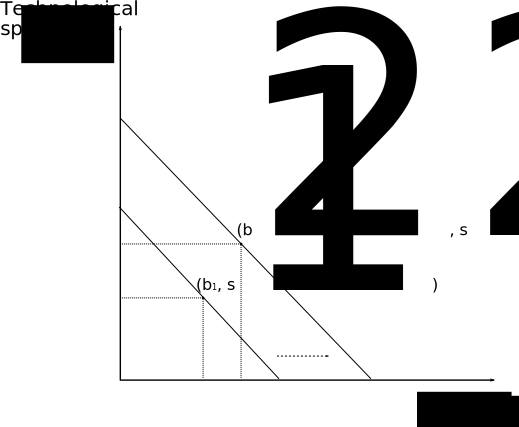
\includegraphics[width=0.75\textwidth, height=0.75\textheight,keepaspectratio]{../figure/budget_constraint}
    \caption{When an official has more endowment, his budget constraint shifts from left to right. He is now able to afford the $(s_2, b_2)$ bundle, with $s_2 > s_1$ and $b_2 > b_1$.}
    \label{fig:budget_constraint}
\end{figure}

\subsection{Parameter 2: price of spillover and private benefit determines the intercept and the slope of the budget constraint}

Given a fixed amount of endowment, the two intercepts of the budget constraint are determined by the ``price'' of the two goods, i.e. how easily the official can obtain technological spillover and private benefit from the foreign investors. If a good becomes harder to extract from foreign firms, the official can afford less of it and the corresponding intercept shifts inward (\Cref{fig:relative_price}). Alternatively, we can think of the slope of the budget constraint as the relative price of the two goods.

Substantively, the ``price'' of technological spillover depends on both the nature of the sector as well as the absorptive capacity of the local economy, which I define as the presence of private firms that are able to absorb technology from foreign firms.\footnote{I define \textit{private firms} as firms with over 50\% ownership belonging to private domestic individuals, companies, or organizations} Consider two channels through which technological spillover happens. First, private firms enter into the supply chain of foreign firms, improving their productivity by imitating the higher production standards or management techniques of foreign firms. For this to happen, it is necessary to have a wealth of private firms that are technologically capable to enter the supply chain. The feasibility of such outsourcing is also sector-specific, e.g. whether the production process is divisible into units, or whether the technology has matured enough for subcontracting. Second, local employees employed by foreign firms may learn from their experience and transfer that knowledge when they move to private firms. For this to happen, private firms must also be technically advanced enough to make use of and compete for this high quality labor from the foreign sector.

The ``price'' of private benefit substantively means how easily the government officials can extract these benefits from the foreign firms. One example of such parameter is the origin of the foreign firm. Firms that come from countries where corruption is more common or accepted would be more adept at providing private benefit to official and more willing to do. In contrast, firms from countries that have signed onto the OECD anti-bribery convention would be more hesitant to bribe given the punishment that they may face from their home governments.

Changing prices of the two goods will shift the budget constraint and, holding the indifference curve constant, have implications for the mix of two goods that the official chooses.

\begin{figure}[!ht]
	\centering
    \includegraphics[width=\textwidth, height=\textheight,keepaspectratio]{../figure/absorptive_capacity}
    \caption{In the left panel, the intercept for private benefit moves from the right to the left as its price increases. In other words, $\frac{E}{p_{b2}} < \frac{E}{p_{b1}}$ because $p_{b2} > p_{b1}$. Similarly, in the right panel, as it becomes more difficult to extract spillover from foreign firms, the intercept moves down.}
    \label{fig:relative_price}
\end{figure}

\subsection{Parameter 3: The official's time horizon determines the shape of his indifference curve}

The official has a convex indifference curve, meaning that there is decreasing marginal utility to both spillover and private benefit. This assumption is standard and makes intuitive sense. As the official accumulates more private benefit, there are fewer things worth spending on as his consumption is satiated and produces less utility. Similarly, when more technological spillover happens, it becomes less of a bottleneck to the economy. Thus, voters (or the official's higher-ups) become less concerned with the issue and it brings less electoral (or career) benefits.

The shape of the indifference curve denotes the relative weight the official assigns to the two goods, spillover and private benefit. When the curve is steep, it means that the official is willing to trade a lot of spillover for a small increase in private benefit. Vice versa, a flatter curve indicates that the official values spillover more (\Cref{fig:indifference_curve}).

Politically, the steepness of the indifference curve depends on the time horizon of the official. This is because technological spillover takes time to happen and increase economic growth whereas private benefit is immediate. The longer the time horizon, the more heavily does he weigh technological spillover effect. For example, in \Cref{fig:indifference_curve}, the blue indifference curve is flatter and signifies more weight assigned to spillover. In that case, the official chooses a bundle that has more spillover and less private benefit (i.e. $s_1 > s_2$ and $b_1 < b_2$). Political factors that influence the official's time horizon may include term limit, the stability of the regime, or the probability of electoral success. 

\begin{figure}[!ht]
	\centering
    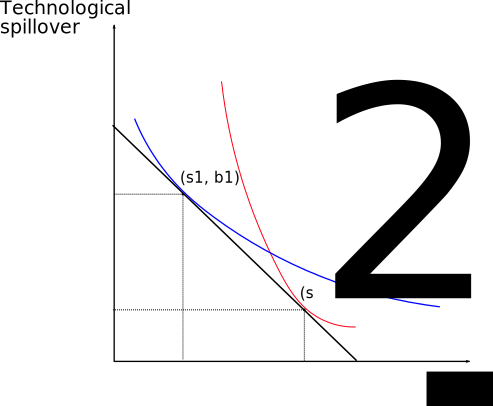
\includegraphics[width=0.75\textwidth, height=0.75\textheight,keepaspectratio]{../figure/indifference_curve}
    \caption{The blue indifference curve shows that the longer the official's time horizon, the flatter his indifference curve, and he will choose more spillover and less private benefit.}
    \label{fig:indifference_curve}
\end{figure}

\subsection{Literature on corruption and FDI}

Regarding private benefit for the officials, I focus on corruption, i.e. bribe and informal fees, given the ubiquity of the practice in developing markets and wealth of data collected on this issue from cross-national business surveys. 

The majority of literature on the relationship between corruption and FDI focuses on showing that a high level of corruption deters FDI \citep{Wei2000, Hakkala2008, Al-Sadig2009}. A smaller literature examines the behaviors of foreign firms that choose to invest in a highly corrupt environment. It argues that foreign firms can help reduce corruption in host country via regulatory pressure effect, demonstration effect, and professionalization effect \citep{Kwok2006}; or via competing away the rents of the domestic firms, reducing the supply of bribes \citep{Sandholtz2003}. In these works, corruption between the host government and the foreign firm has been conceptualized as \textit{predatory}.

My research offers a new perspective, recognizing that, compared to domestic firms, foreign firms always have the freedom to move out of the country or at least stop bringing in capital. Therefore, the exchange between the government and foreign firms are always more voluntary compared to private firms. In this angle, corruption between the government and the foreign firm can be \textit{collusive}, with government officials getting bribe and foreign firms getting exclusive access to resources controlled by the officials (e.g. an expedited bureaucracy or privileged use of public resources) \citep{Hellman2002}. Indeed, there are evidence of foreign firms bribing to get an upper hand in the local market \citep{Barstow2012} or to pursue rent in protected industries \citep{Malesky2015}. 

Such collusive corruption between the government and foreign firm can be the key to explain the puzzle why governments may want to attract a lot of FDI despite the lack of developmental impact. (Corrupt) institutions matter, but not only to \textit{how much} FDI a country can attract as the literature has studied, but also \textit{which kind}.


\subsection{Road map}

In the sections that follow, I contextualize the general theory presented above, building three mid-level theories that map each of the three parameters to a specific empirical context. I also briefly discuss the identification strategy, leaving more operationalization and data availability details for the later Research Design section.

The three parameters in the model and their empirical implications are:

\begin{itemize}
\item \textit{``price'' of spillover}: sectoral and industry variation in the level of potential spillover affects the official's choice of the spillover-bribe bundle.

\item \textit{``price'' of private benefit}: Phase 3 enforcement of OECD's anti-bribery convention makes firms from member countries more hesitant to bribe, raising the cost of bribery and resulting in less bribe and more spillover.

\item \textit{time horizon}: term limit reduces the time horizon of Vietnamese provincial officials that are close to retirement, leading to less spillover and more bribery.
\end{itemize}

\end{document}